%
% Chapter 3
%
% Response eQTL-style paper

\chapter{Genetic factors affecting Pandemrix vaccine response}
\label{chap:hird_reQTL}

\section{Introduction}

\subsection{Genetic factors affecting influenza vaccine response}

- Vaccine-induced antibody response is a complex trait.
% Impact of host genetic polymorphisms on vaccine induced antibody response
% https://www.ncbi.nlm.nih.gov/pmc/articles/PMC4962936/#!po=22.7273
% Table 1.
% Genes with polymorphisms that influence the vaccine induced antibody level (selected studies).
% Individuals carrying the minor allele in one or both alleles showed an increased seroconversion rate after influenza vaccination.62
% Further SNPs that influence the humoral immune response to influenza vaccination have been reported (see Table 1):

Specifically for response to seasonal influenza vaccines...
% Start here with this review
% 2019
% Host Factors Impact Vaccine Efficacy: Implications for Seasonal and Universal Influenza Vaccine Programs
% https://jvi.asm.org/content/93/21/e00797-19

% 2004
% HLA-DRB1*0701 allele was over represented among persons who fail to mount a neutralizing antibody response.
% https://www.ncbi.nlm.nih.gov/pubmed/15462607

% 2008
% Immunogenetics of Seasonal Influenza Vaccine Response
% https://www.ncbi.nlm.nih.gov/pmc/articles/PMC2610683/

% 2019
% Common Genetic Variations Associated with thePersistence of Immunity following ChildhoodImmunization
% https://www.cell.com/cell-reports/pdf/S2211-1247(19)30682-5.pdf

% Stretch?
% Also
% Prevacc signatures of Tri
% Using larger transcriptomic dataset
% Are they genetic

\subsection{\Glsfmtlongpl{reQTL} for seasonal influenza vaccination}

A potential mechanism through which genetic variation can affect vaccine response is through altering the expression of genes.

eQTLs have condition specificity
e.g. cell types or tissues

A reQTL is: \autocite{vandiedonck2017GeneticAssociationMolecular}
% An important kind of eQTLs, called response eQTLs (reQTLs), occurs following
% exposure to an external signal (Table 2), in particular in the immune system in
% response to infectious agents and to various stimuli.49, 54, 55 Other
% environmental factors, including hormones, drugs, diet, metals or pollutants,
% can also be the source of reQTLs.56
- an eQTL becomes more or less important after perturbation: Tells you something about the mechanism of perturbation.
- Either expression regulatory activation/repression (signalling cascade -> TFs, chromatin remodelling etc.)

Little work done on reQTL for vaccine stimulation
Summarise Franco et al
In the case of inactivated trivalent influenza vaccine, genetic variation in membrane trafficking and antigen processing genes was associated with both transcriptomic and antibody responses in patients after vaccination [Franco].

\subsection{Chapter summary}

% NOTE:
% Narcolepsy controversy (more evidence for genetic interaction with Pandemrix vaccine response in particular)

- In \autoref{chap:hird_DGE}, we observed massive changes in gene expression longitudinally after Pandemrix vaccination, as well as expression signatures correlated to degree of antibody responses.
[variation observed in response to Pandemrix, e.g R vs. NR trajectories]
- How does host genetics affect response to Pandemrix in the HIRD cohort?

Sobolev pros
    Small effect expected?
    More variation will usually be explained by history of exposure rather than genetics, so may be harder to detect.
    but not here

also Knowns
    Sobolev: R vs NR, 
    inconsistent variation in why people are NR

In this study, we model the influence of host genetics on longitudinal transcriptomic and antibody responses to Pandemrix, in vivo.
    overall strat: map per timepoint, joint analysis
    call reqtls
    characterise
% have abs
    % not that we use
% [main aim: how much variation in response is genetic?]
    % not that we calc
% [other aims: assess differences to seasonal influenza vaccines]
% [summary of main results]
% Utility of genetics: allows coloc

\section{Methods}

\subsection{Overall strategy for detecting reQTLs}

% TODO: start here. text!

for reQTL
it may also seem natural
overall Why not mapping on deltas? (if we are interested in the direct question of G on change)
    ackermann: change scores are prone to increased noise
    from franco: "We attempted analyses with an approach similar to that proposed by the reviewers in the course of our work, but found that the approach that was ultimately chosen to explore the day differences was the most powerful. Specifically, utilizing a pairwise comparison (difference) between time points as the substrate for the eQTL analysis would lead to an increase in the technical variance of the phenotype, as the sum of two independent (technical) errors has twice the variance of an individual measurement. "

instead within timepoint, and compare effects
if change in expression vs d0 is under genetic control, we should see change in effect size of eqtl vs d0
can do this because genotype can be assumed to be constant across timepoints

It can be a tricky business to define response eQTLs, or indeed any condition specific eQTLs
    early attempts
    naive
    map condition by condition
    signif

why joint
In the same period that condition specific eQTL mapping was getting started (as discussed in section...), tools were being created to identify these locitools were being created to identify these loci
review: condition/Cell-type specific methods
refere to 2019-11-19 Cell-count specific eQTL mapping papers
PANAMA, LIMMI

%
% Restricted to non-full Bayesian methods.
%
% See last paragraph of discussion in
% Kontopantelis, E., Springate, D. A., & Reeves, D. (2013). A Re-Analysis of the Cochrane Library Data: The Dangers of Unobserved Heterogeneity in Meta-Analyses. PLoS ONE, 8(7), e69930. https://doi.org/10.1371/journal.pone.0069930
% For small k, Sidik MVa or Ruhkin RBp recommended.
%
% metafor manual
% If, instead of the crude estimate, one wants to use a better apriori estimate, one can do so by passing this value via control=list(tau2.init=value)
% Sidik-Jonkman estimator, also called the ‘model error variance estimator’, is implemented in metafor (SJ method).
% Starts with an init estiamte of ri=sigma2i/tau2i i.e. ratio of study-specific and between-studies het variance, then updates.
% They recommend using Hedges [1], to init, but this is bad???
% We use mode of gamma as an apriori estimate of tau.
%
% 2.7.	Meta-analysis with metafor
% 2.7.1.	Per day, use rma(‘REML’) to fit random-effects model on association beta and beta_ste, per gene-SNP pair, using all timepoints from array/RNA-seq for that day
% 2.8.	eigenMT to get number of independent tests per gene
% 2.8.1.	split previously generated geneloc and snpsloc by chrom
% 2.8.2.	per chrom, run eigenMT on limix output (arbitrary day, since the set of snps cis to each gene does not vary by day)
% 2.9.	Compute hierarchical FDR
% 2.9.1.	Per day
% 2.9.1.1.	Use eigenMT estimates to apply local Bonferroni per gene
% 2.9.1.2.	Compute global BH FDR

Finally
recall hird has multi datasets and measures within each timepoitn

why mega?
    can't bayesmeta, which would be ideal.
    also, small n for array


\subsection{Mapping cis-\glsfmtlongpl{eQTL} with \glsfmtlongpl{LMM}}

As discussed in \autoref{chap:hird_DGE}, the \gls{HIRD} cohort is multi-ethnic, and population structure can affect gene expression\autocite{brown2018ExpressionReflectsPopulation}.
I addressed this by treating the top \glspl{PC} of the genotype matrix as covariates for large-scale population structure (ancestry).
In the context of \gls{eQTL} mapping, where the aim is to assess the marginal effect of a single genetic variant on expression, it is even more important that the confounding effect of population structure is accounted for.

% This is great background/intuition: golan2018MixedModelsCaseControl
% using LMMs is appropriate for controlling for population structure (which is a common
% problem in human GWAS), as well as for cryptic relatedness, and that LMMs outperform
% the previously preferred principal component analysis (PCA) approach in addressing these
% issues (Yang et al., 2014).
%
% Also see: 2018-11-26 notes in log
For genetic association studies, an appealing approach is the \gls{LMM}, which includes a random effect that directly models genetic correlation between individuals as the covariance of that random effect\autocite{price2010NewApproachesPopulation, eu-ahsunthornwattana2014ComparisonMethodsAccount, golan2018MixedModelsCaseControl}
The \gls{LMM} approach has the advantage of not only modelling large-scale population structure, but also cryptic relatedness (the presence of closely related individuals in a sample assumed to consist of unrelated individuals\url{https://projecteuclid.org/euclid.ss/1271770342}) from finer-scale effects such as family structure\autocite{golan2018MixedModelsCaseControl}.
\todo{add some indication of how much inflation is reduced by LMMs}

\subsubsection{Estimation of kinship matrices}

% 1.	Build GRM using LDAK 5
% 1.1.	Start with pre-imputed genotypes coreex_eQTLflu_20171204.gencall.smajor.impute_sex.qc6
% 1.1.1.	“Estimates of SNP heritability are very sensitive to genotyping errors”, so we can’t use imputed SNPs without filtering for high INFO.
% 1.2.	Prune to MAF 0.05, autosomes only
% 1.3.	Compute LDAK SNP weightings
% 1.4.	Compute kinships for each chromosome
% 1.5.	Join per-chromosome kinships into genome-wide kinships
% 1.5.1.	Use the leave-one-chromosome-out strategy

- The LMM requires a kinship matrix to scale(?) the covariance matrix of the random effect
- When testing a variant for association, to avoid loss of power from 'proximal contamination', kinship matrix used should not include that variant\url{https://www.ncbi.nlm.nih.gov/pmc/articles/PMC3597090/}.
- A simple way to avoid this is to compute \gls{LOCO} kinship matrices from all variants on chromosomes other than that variant's chromosome\autocite{lippert2011FaSTLinearMixed}.

I estimated kinship in the \gls{HIRD} data from common autosomal variants, using \texttt{LDAK} (5.0), which computes kinship matrices adjusted for bias caused by \gls{LD}\autocite{speed2012ImprovedHeritabilityEstimation}.
Filtered, pre-imputation sample genotypes from \autoref{subsec:hird_DGE_methods_genotypePhasingAndImputation} were pruned to $\text{\gls{MAF}} > 0.05$.
A kinship matrix was computed for each autosome, then combined into a single genome-wide matrix using \texttt{LDAK -{}-join-kins}.
To obtain a \gls{LOCO} kinship matrix for each autosome, each autosome's kinship matrix was then subtracted from this genome-wide matrix (\texttt{LDAK -{}-sub-grm}).
- The \gls{LOCO} kinship matrix excluding chromosome 1 is shown [...]

\missingfigure{chr1 loc kinship matrix as example, note the estimates for self-relatedness on the diagonals are not constrained to be 1.}

% Full notes about cell type correction pipeline rationale at 2019-10-30 in log
\subsubsection{Estimation of cell type abundance via expression deconvolution}

As \gls{PBMC} samples are a mixture of immune cells, and a fixed input of RNA extracted from that mixture is used to estimate expression, bulk estimates for genes that have cell type specific expression depend on the relative proportions of each cell type in each sample.
% Also, \gls{RNAseq} expression estimates are inherently compositional \url{https://www.ncbi.nlm.nih.gov/pubmed/29608657} \url{https://academic.oup.com/gigascience/article/8/9/giz107/5572529}.

% E.g. Davenport 2018: “observed eQTL interactions could be the consequence of a cellular subpopulation whose frequency is being altered by the environmental perturbagen or variability in cell type proportions between individuals.”
% “inferred the relative proportions of nine hematopoietic populations from the RNA-seq data using CIBERSORT”
% After correcting for cell proportions “reduction in significant interactions suggests that some of these interactions may be related to changes in cell proportions”
- G is constant. C is not constant
- It is well known that QTLs can be cell type specific, due to cell type specific expression and other mechanisms (fu)
- Cell proportions change after vacc, reQTLs calls can be confounded if cell type abundances are not taken into account.
- If it is assumed that eQTL effects can differ between cell types, then in addition to the genotype main efect, an interaction term between genotype and cell type abundance is required.

- Need an estimate of abundance.
- I do not have FACS data for all samples in HIRD, only subset of array individuals.
% Related:
% Westra, H.-J., Arends, D., Esko, T., Peters, M. J., Schurmann, C., Schramm, K., … Franke, L. (2015). Cell Specific eQTL Analysis without Sorting Cells. PLOS Genetics, 11(5), e1005223. https://doi.org/10.1371/journal.pgen.1005223
% Gets cell type estimates from proxy genes
- Expression deconvolution is a viable alternative.
- Chose xCell, as used by the GTEx paper, which works by... e.g. spillover etc. ... returns enrichment scores which are not... only uses about 10k genes
- xCell includes signatures for 64 cell types, but recommends cell types not be included if not expected to be present.
% See 2019-11-14 log
% https://link.springer.com/chapter/10.1007/978-3-319-16104-4_15
% https://www.nature.com/articles/s41588-018-0089-9
% www.blueprint-epigenome.eu/index.cfm?p=7BCEDA45-EC73-3496-2C823D929DD423DB
Reviewing the literature to find broad classifications for peripheral blood cell types also present in the \gls{PBMC} compartment\autocite{davenport2018DiscoveringVivoCytokineeQTL},
I settled on 'CD4+ T-cells', 'CD8+ T-cells', 'B-cells', 'Plasma cells', NK cells, Monocytes and DCs.

xCell applied to expression data 
% /nfs/users/nfs_b/bb9/workspace/phd/output/hird/rnaseq/4_de/array/array_data_setup.y.filtered.MaxMean.combat.rds
% and /nfs/users/nfs_b/bb9/workspace/phd/output/hird/rnaseq/4_de/array/array_data_setup.sample.metadata.merged.rds
As xCell is rank-based, no additional xforms.
rnaseq and array separate

- xCell enrichment scores scaled and centered, 
- Scale all timepoints together, so that a value of 0 cell proportion effect represents the same thing across all timepoints

\begin{figure}
    \centering
    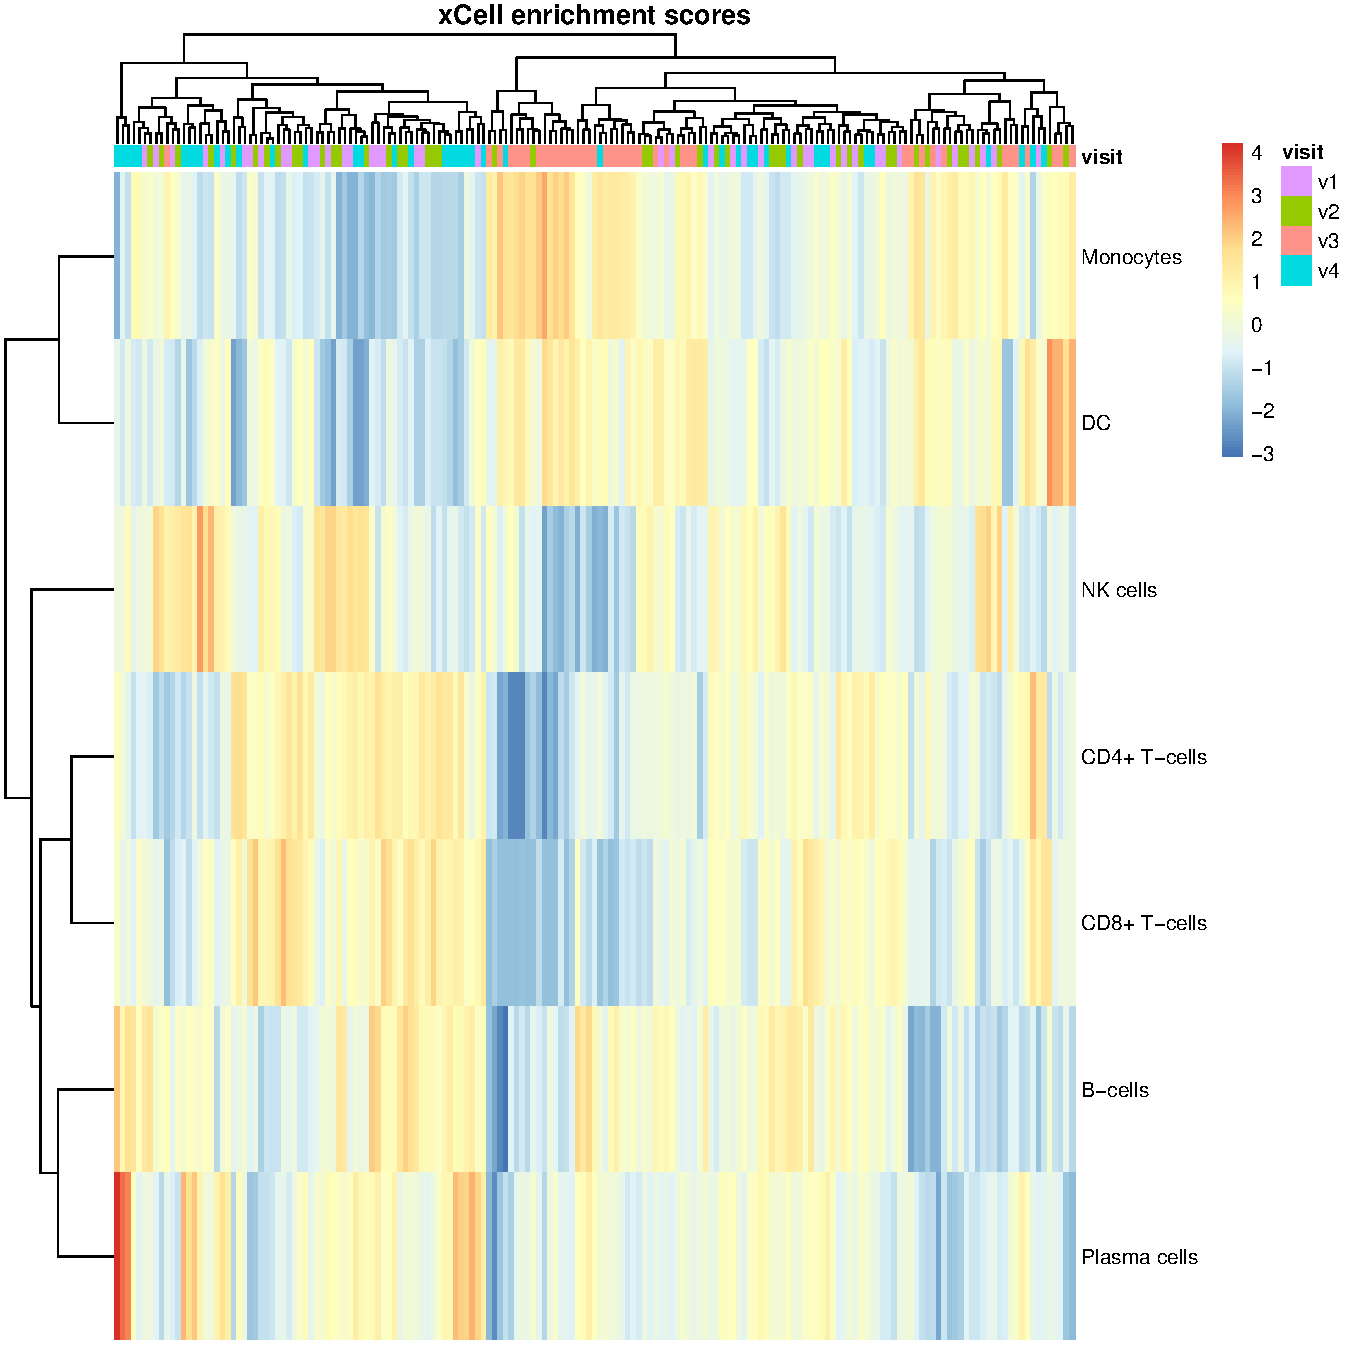
\includegraphics[width=1.0\textwidth,page=1]{mainmatter/figures/chapter_03/get_xCell_estimates.dataset_array.plots.pdf}
    \caption{xCell enrichment scores in array data}
    \label{fig:hird_xCell_scores_heatmap_array}
\end{figure}

\begin{figure}
    \centering
    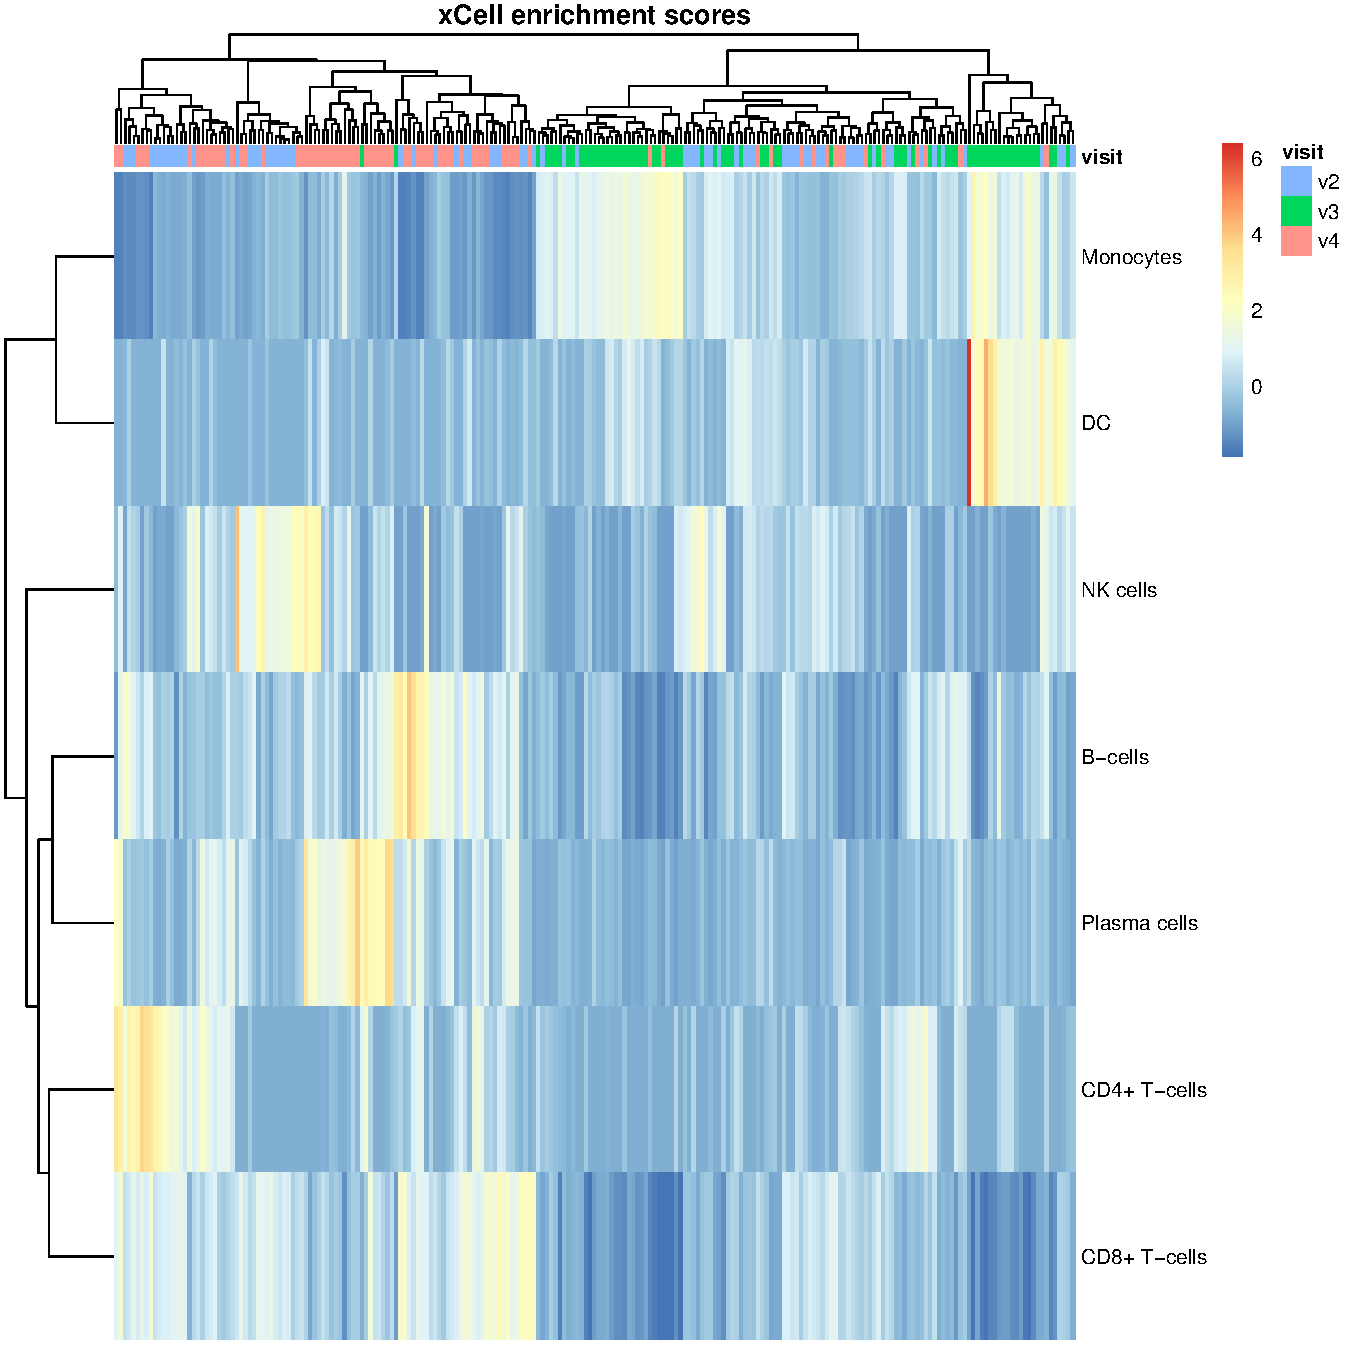
\includegraphics[width=1.0\textwidth,page=1]{mainmatter/figures/chapter_03/get_xCell_estimates.dataset_rnaseq.plots.pdf}
    \caption{xCell enrichment scores in rnaseq data}
    \label{fig:hird_xCell_scores_heatmap_rnaseq}
\end{figure}

- The xCell estimates are correlated.
- select top ones that are reasonable uncorrelated
- in each case 3 pcs pass eigenvalue > 1 rule of thumb
- PCA them
PCs are orthogonal (and thus linearly independent)
but for intepretability
- select top 3 cell types with close cos2
    - they are also top cells that changed in sobolev


\begin{figure}
    \centering
    \begin{subfigure}[b]{0.49\textwidth}
        \centering
        \includegraphics[width=1.0\textwidth,page=8]{mainmatter/figures/chapter_03/get_xCell_estimates.dataset_array.plots.pdf}
        \caption{array}
    \end{subfigure}%
    \hfill%
    \begin{subfigure}[b]{0.49\textwidth}
        \centering
        \includegraphics[width=1.0\textwidth,page=8]{mainmatter/figures/chapter_03/get_xCell_estimates.dataset_rnaseq.plots.pdf}
        \caption{rnaseq}
    \end{subfigure}%
    \caption{xCell cos2 contributions}
    \label{fig:hird_xCell_loadings}
\end{figure}


% NOTE:
% Why impute for cell counts but not for expression data?
% - expression matrices are mostly complete, and we only exclude genes based on low expression in RNAseq
% - we cannot drop whole FACS panels so easily like we can drop genes
- Validate estimates on subset with FACS data.

-    group raw data by panel and cell type
-    Rank-Based Inverse Normal Transformation
    % PHEASANT https://www.biorxiv.org/content/biorxiv/early/2017/02/26/111500.full.pdf and
    % Astle 2016, both use this method.
- then imputewithmissForest


- plot against xcell estimates
- kinda moderate, esp at day1

\begin{figure}
    \centering
    \begin{subfigure}[b]{0.43\textwidth}
        \centering
        \includegraphics[width=1.0\textwidth,page=6]{mainmatter/figures/chapter_03/validate_xCell_estimates.cell_type_pairs.pdf}
        \caption{mono}
    \end{subfigure}%
    \vspace{1em}\vfill%
    \begin{subfigure}[b]{0.43\textwidth}
        \centering
        \includegraphics[width=1.0\textwidth,page=3]{mainmatter/figures/chapter_03/validate_xCell_estimates.cell_type_pairs.pdf}
        \caption{nk}
    \end{subfigure}%
    \vspace{1em}\vfill%
    \begin{subfigure}[b]{0.43\textwidth}
        \centering
        \includegraphics[width=1.0\textwidth,page=2]{mainmatter/figures/chapter_03/validate_xCell_estimates.cell_type_pairs.pdf}
        \caption{plasma}
    \end{subfigure}%
    \caption{xCell vs facs int}
    \label{fig:hird_xCell_vs_FACS}
\end{figure}

\subsubsection{\glsfmtshort{eQTL}-specific expression preprocessing}

There are a wide range of transformations that are often applied to expression data before \gls{eQTL} mapping.

e.g. Rank-based int:
% 2018-03-15 in log details the GTEx pipeline.
heavily used in eqtl, e.g GTEX \url{https://storage.googleapis.com/gtex-public-data/Portal_Analysis_Methods_v7_09052017.pdf}
    Although criticised: "Rank-Based Inverse Normal Transformations are Increasingly Used, But are They Merited?"

e.g. Z
\url{https://github.com/molgenis/systemsgenetics/wiki/eQTL-mapping-analysis-cookbook-(eQTLGen)}

- outliers
- normality also: genomic data: resid normal is mostly defined by input normal

- Considering my main goal is to find reQTLs
I performed simulations to evaluate the effect of the transformation on reQTL calls

sim reQTLs on the log scale with specific betas
define strength as diff

scale only
2 and 4 sim to have same relative effect size change
2 and 4: betas are 0 1, 1 2
after, 0 0.75, 0.4, 0.8

only center
both
do not induce fals negs
preserve both rel egene str

but no point, since intercept is included

in the end, no scale
extra careful on outliers

\begin{figure}
    \centering
    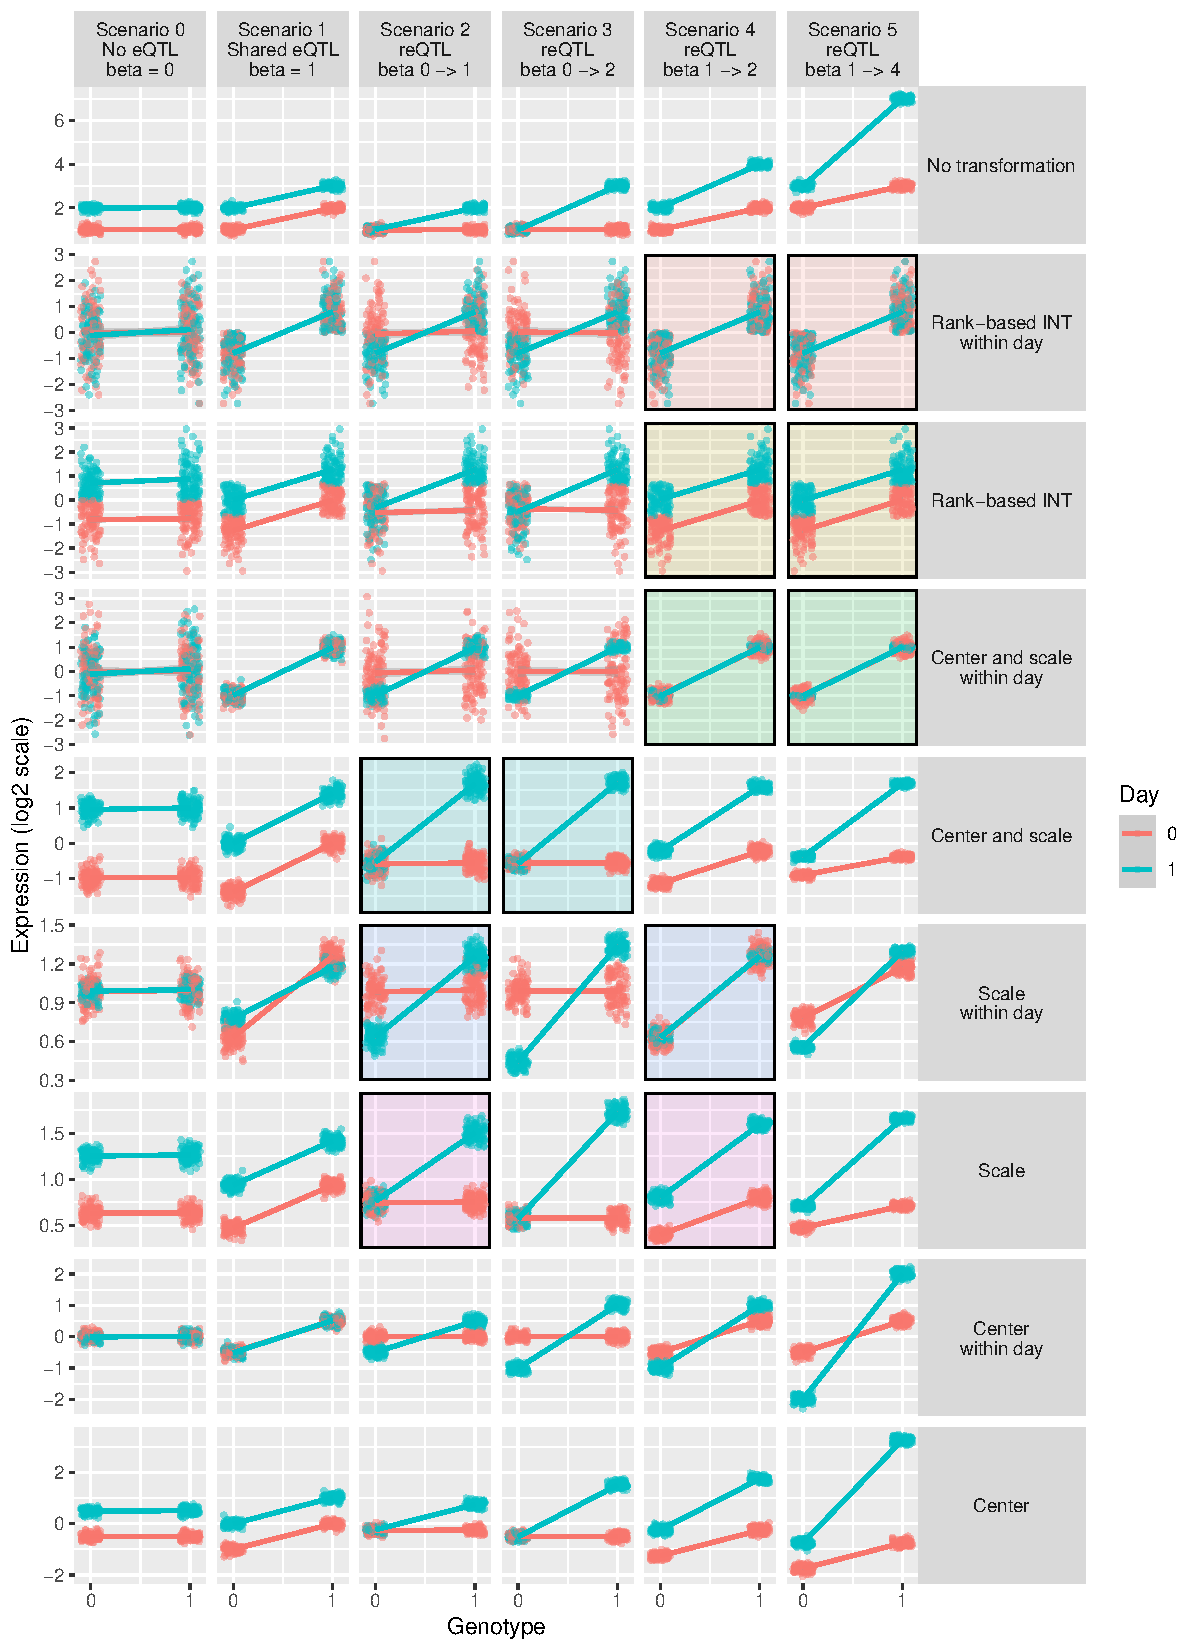
\includegraphics[width=1.0\textwidth,page=1]{mainmatter/figures/chapter_03/simulate_expression_transforms.pdf}
    \caption{expression xforms}
    \label{fig:hird_eQTL_expressionTransform_sims}
\end{figure}

\subsubsection{Finding hidden confounders using factor analysis}

% 2.	Infer global confounders by detecting hidden factors affecting expression with PEER
% 2.1.	“batch effects and other global confounders reduce the power to find expression quantitative trait loci”
% 2.1.1.	“We assume that these variables have a broad influence, and thus each of them has an effect size for every gene.”
% 2.1.2.	“The learned variables can be constrained to affect known sets of genes via a prior connectivity matrix. By default, with no prior connectivity given, they are assumed to be global and to affect large fractions of all genes“
% 2.1.3.	Note that due to this assumption: “If large trans hotspots are dominating, associations may get erroneously explained away as confounding factors”
% 2.2.	Round input expression to integer counts
% 2.2.1.	Input is y: the scaledTPM (TPM's scaled up to library size) from tximport.
% 2.3.	Normalise for library size and variance stabilize with varianceStabilizingTransformation from DESeq2 (recommended in PEER paper)
% 2.3.1.	Vst is like a souped up log: “In all cases, the transformation is scaled such that for large counts, it becomes asymptotically (for large values) equal to the logarithm to base 2 of normalized counts.”
% 2.3.2.	Note we cannot use voom-ed expressions from the DGE pipeline, as there are some samples missing due to lack of Ab titre data
% 2.3.3.	Do not blind the transformation to experimental design matrix: “If many of genes have large differences in counts due to the experimental design, it is important to set blind=FALSE for downstream analysis.”
% 2.3.4.	Here we use a simple design matrix of groups defined by all combos of day x R/NR
% 2.4.	Run PEER by timepoint
% 2.4.1.	Match GTeX pipeline: https://github.com/broadinstitute/gtex-pipeline/tree/63b13b8ced25cf8ab8e7a26f40a495e523630a9b/qtl , with some modifications.
% 2.4.1.1.	Note this pipeline uses quantile normalized, rank INT transformed expression, as PEER input
% 2.4.2.	Quantile normalize the samples with preprocessCore::normalize.quantiles
% 2.4.2.1.	Causes the expressions of the samples to have the same empirical distribution
% 2.4.2.2.	i.e. the the highest expression in each sample is set to the mean of the highest values of all samples, and in the case of no tied values, each sample’s expressions becomes a permutation of each other sample’s
% 2.4.3.	Standardize expression of each gene with Rank-Based Inverse Normal Transformation
% 2.4.3.1.	i.e. rank the expressions of a gene, then replace with values from the standard normal e.g. > rank.based.INT(1:5, c=3/8): [1] -1.1797611 -0.4972006  0.0000000  0.4972006  1.1797611
% 2.4.4.	Setup and run PEER
% 2.4.4.1.	Allow up to 10k iterations, start with n.samples/4 PEER factors
% 2.4.4.2.	One can include known covariates. We don’t, as it causes weird things like PEER factors not being sorted in descending relevance
% 2.4.4.2.1.	~ 1 + batch + rna.conc + Gender + Age.at.vaccination..years. + PC1.imputed + PC2.imputed + PC3.imputed + PC4.imputed
% 2.4.4.2.2.	Note this includes an intercept that represents the mean expression

myriad of other fx are not constant

PEER

% If RANKINT, why RANKINT before PEER?
%
% Are your covariates under control? How normalization can re-introduce covariate effects
% https://www.ncbi.nlm.nih.gov/pubmed/29706643
% "Many statistical tests rely on the assumption that the residuals of a model are normally distributed [1]. In genetic analyses of complex traits, the normality of residuals is largely determined by the normality of the dependent variable (phenotype) due to the very small effect size of individual genetic variants [2]. However, many traits do not follow a normal distribution."
% "applying rank-based INT to the dependent variable residuals after regressing out covariates re-introduces a linear correlation between the dependent variable and covariates, increasing type-I errors and reducing power."


% Trans-eQTLs Reveal That Independent Genetic Variants Associated with a Complex Phenotype Converge on Intermediate Genes, with a Major Role for the HLA
% https://doi.org/10.1371/journal.pgen.1002197
%
% In order to increase the number of detectable cis- and trans-eQTLs we applied a
% principal component analysis (PCA) on the sample correlation matrix. We, among
% others [19], [20], argue that the dominant PCs, capturing the larger part of
% the total variation, will primarily capture sample differences in expression
% that reflect physiological or environmental variation as well as systematic
% experimental variation (e.g. batch and technical effects).
% [...]
% An aspect to consider is that with
% the removal of more PCs from the data, the degrees of freedom of the data will
% decrease. Furthermore, it is not immediately clear which PCs will actually
% capture physiological, environmental, and systematic variation, which might
% lead to removal of genetically determined expression variation as well.
% Therefore a tradeoff has to be made on the number of PCs to subtract from the
% data.
% - subtracted 50 PCs for cis, 25 PCs for trans.

expression PCs: if too many, will explain away the signal
Not a problem with cis-eQTLs, but trans might have more global effects
    GWAS on PEER factors would pick up trans fx, cell count QTL effects
Unlike PCs, PEER factors are not constrained to be orthogonal: adding more and more factors will not explain more of the variance
    Also, they are weighted with ARD 
    results is that variance of output factors declines to zero

start with COUNT Data

convert to log scale and var stab
RNAseq only
% vsd <- vst(dds.filtered, blind=F)
mega
% vsd <- ComBat(dat=vsd, batch=sample.metadata.merged$batch, par.prior = T)
vsd is a log with shrinkage for low counts
also corrects for depth between sampline norm

gender, 4pcs, 3 cell types
explicit inclusion, peer finds additinal k

why include genetic PCs
see stegle 2012 PEER paper: if PCs are not included, they can be recapitulated in the factors
% (e.g., by introducing principal components of the genotype data), is not included in the model, and it may be recapitulated in the inferred factors.

\subsubsection{\glsfmtshort{eQTL} mapping per timepoint}

% 2.5.	Preprocess genotypes for limix
% 2.5.1.	Convert MAF filtered VCF -> 012 -> hdf5 format
% 2.5.1.1.	Do this for both strict 012 and continuous dosages
% 2.5.2.	Also convert 012 -> matrix eqtl SNP matrix format
% 2.5.2.1.	For eigenMT
% 2.5.3.	Parse out snpinfo and snplocs from VCFs
% 2.5.3.1.	Snpinfo for snp ids, for limix
% 2.5.3.2.	Snplocs for snp positions, and eigenMT
% 2.6.	Map eQTLs using limix 2.0, per timepoint
% 2.6.1.	Map cis-eQTLs within +- 1Mb of the gene start
% 2.6.1.1.	Phenotypes: per timepoint normalised input.expr from PEER script
% 2.6.1.2.	Covariates: sex, batch, 4 genotype PCs, 4 PEER factors
% 2.6.1.3.	Genotypes: MAF > 0.10 (in whole 169 individuals)
% 2.6.1.4.	Kinship: from LDAK, leave-one-chrom-out
% 2.6.2.	Output results in matrix eqtl-like output format

% For list of various methods considered, also see 2018-03-05, 2018-07-25, 2018-07-27 etc. in log
The performance of various software implementations of \glspl{LMM} specialised for genetic association studies are highly comparable; the specific choice of implementation can usually be made on the basis of computational efficiency\autocite{eu-ahsunthornwattana2014ComparisonMethodsAccount}.

choose the covariates approach, not residuals
    % Bias due to two‐stage residual‐outcome regression analysis in genetic association studies https://doi.org/10.1002/gepi.20607
    why including known covariates: why not a two stage approach?

    as sample size is modest, keep dfs correct
    how to choose number?

\begin{figure}
    \centering
    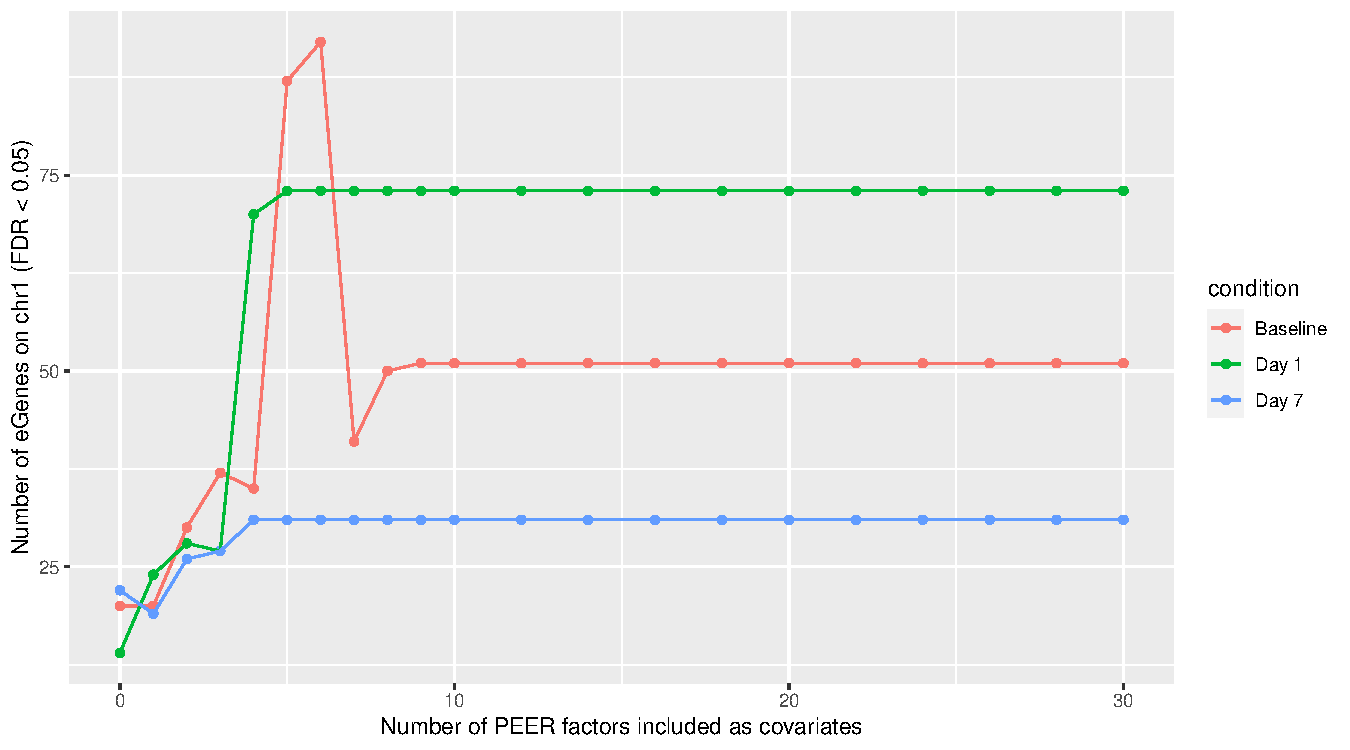
\includegraphics[width=1.0\textwidth,page=1]{mainmatter/figures/chapter_03/count_eGenes.signif_eGenes_vs_PEER_n.dataset_mega.chr_chr1.pdf}
    \caption{optimlise}
    \label{fig:hird_neGenesvsPeerK}
\end{figure}

var filters

    Sample AC thresh
        note they are dosages. if they were not, use ac thresh to estimate number of hom minor expected

    Partial justification for not considering sex chromosomes
    % https://www.nature.com/articles/ng.467
    % As is standard for imputation, we excluded all X-linked SNPs for the following reasons: (i) the X chromosome has to be treated differently from the autosomes; (ii) it cannot be predicted which allele is active on the X chromosome, (iii) testing males separately from females results in different sample sizes and power. Imputation of SNPs in the HapMap CEU population was performed using either MACH46 or IMPUTE47. All SNPs with a MAF <0.01 were excluded from analysis. In total, up to 2.11 million genotyped or imputed SNPs were analyzed.

Post-impuation, Genotypes are probabilities
    Genotypes were converted to dosages using bcftools (1.7-1-ge07034a)

The final model:

% sample_AC_thresh 15
% cis_dist 1e6
% cis only

% x genes

\subsection{Joint \glsfmtshort{eQTL} analysis across timepoints}

% 2.10.	mashr
% 2.10.1.	Apply mashr to per-day meta-analysis beta/beta_ste results

Simple, mixed models, joint models, multilocus models; Ending with why we chose mashr
used for smoothing, info sharing, fdr
    normally eqtls use perms for FDR
mashr beats out stuff it compared to in the paper e.g. metasoft

fit model

Choice of strong effects
If there is a particular condition with much greater power, choosing the lowest p value for each gene across all conditions could bias strong effects towards including just condition-specific effects for that particular condition.
how to ensure condition specific effects are present? look at heatmap of strong subset

correlations
    we dont' give up repeat measures strenght

compute posteriors

lfsr:
% type s error rates for classical and bayesian single and multiple comparison procedures
% WhyWe (Usually) Don’t Have to Worry About Multiple Comparisons (2012)
% Beyond Power Calculations: Assessing Type S (Sign) and Type M (Magnitude) Errors (2014)
% Stephens, M. (2016). False discovery rates: A new deal. Biostatistics, kxw041. https://doi.org/10.1093/biostatistics/kxw041

\subsection{Defining shared and response eQTLs}
% See notes from 2018-10-11 on wald test, and comments on sharing_func in get sharing script

mash suggests, but limitations
% # We define two effects to be shared in sign if they
% # have the same sign; we define them to be shared in magnitude if they also have an
% # effect within a factor of 2 of one another.
% # When computing sharing between tissues r and s, we consider only
% # QTLs that are significant (lfsr < 0.05) in at least one of r and s. This is to avoid
% # sharing estimates being driven by estimates of null or nearly null effects.

beta-comparison approach from Sarah Kim-Hellmuth 2017
% 7 conditions, pairwise
% note they use lead, then correct bonf

% 113             # Also see:
% 114             # https://stats.stackexchange.com/questions/93540/testing-equality-of-coefficients-from-two-different-regressions
% 115             # https://stats.stackexchange.com/questions/55501/test-a-significant-difference-between-two-slope-values
% 116             # http://www.stat.columbia.edu/~gelman/research/unpublished/signif3.pdf
% 117             # USING THE CORRECT STATISTICAL TEST FOR THE EQUALITY OF REGRESSION COEFFICIENTS
% 118             #     https://doi.org/10.1111/j.1745-9125.1998.tb01268.x
% 119             # Schenker, N., & Gentleman, J. F. (2001). On Judging the Significance of Differences by Examining the Overlap Between Confidence Intervals.
% 120             #     http://dx.doi.org/10.1198/000313001317097960
% 121             # https://andrewpwheeler.wordpress.com/2016/10/19/testing-the-equality-of-two-regression-coefficients/
% 122             #     Var(A-B) = Var(A) + Var(B) - 2*Cov(A,B)
% 123             #     NOTE: Assumes that Cov is 0, this is anticonservative when Cov is actually positive.
% 124             #
% 125             # https://www.ncbi.nlm.nih.gov/pmc/articles/PMC5559603/ uses the Z test for beta comparison
% 126             # "This approach is highly consistent with a previously used method6,
% 127             # 8, 10 where differential expression is used as the quantitative trait"

% Why can we use a Z test?
% Very similar to a Wald test. See 2018-10-11 log.

% 217     qtls.merged[, signif_rank := frank(qtls.merged, lfsr, -INFO, -MAF_sample, SNP_gene_TSS_dist, POS)]

NOTE we are not interested in stat signif, this is heuristic threshold for interesting effects

\subsection{Replication of eQTLs in a reference dataset}

- pi1 method

\subsection{Fitting models with interactions}

- lme4qtl method

\section{Results}

\subsection{Per timepoint mapping}

- mapped eQTLs at x genes, x autosomal variants, each timepoitn
- 3 versions
- limix, mashr
- reqtl defined as

- x genes had eQTL at at least 1 timepoint (eGene)
- overall eGene rate in each analysis is

- decide on version: replication
- shared replicates well
- mega superior

\begin{figure}
    \centering
    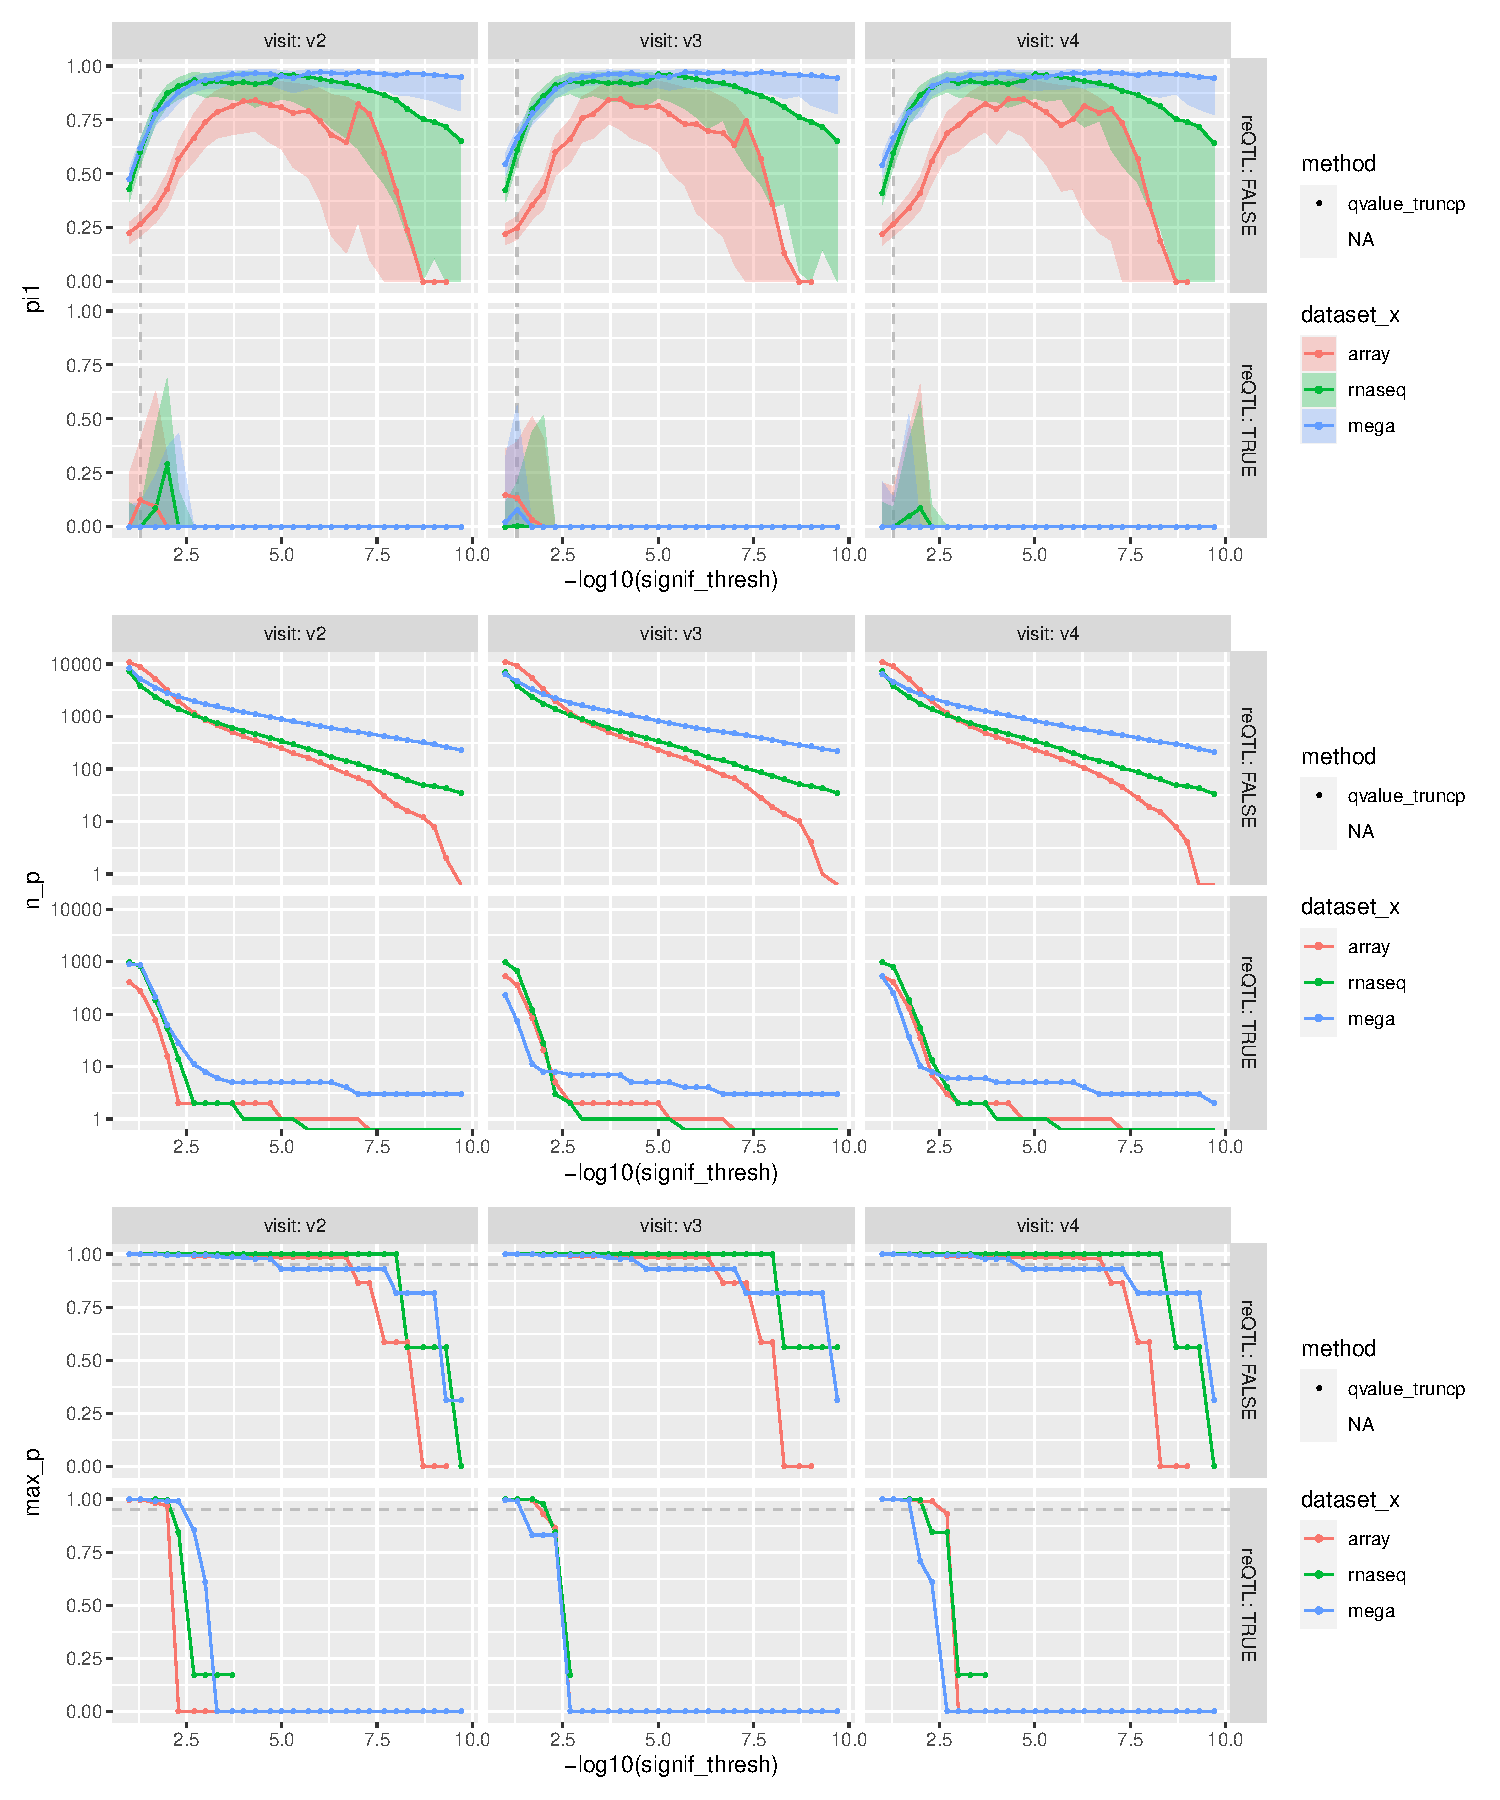
\includegraphics[width=1.0\textwidth,page=1]{mainmatter/figures/chapter_03/compute_pi1.pi1_by_thresholds.pdf}
    \caption{}
    \label{fig:hird_eQTL_pi1vsGTExWholeBlood}
\end{figure}

- more detailed breakdown of sharing in mega
- day 0 more egenes

\begin{figure}
    \centering
    
\includegraphics[width=1.0\textwidth,page=2]{mainmatter/figures/chapter_03/get_signif_qtls.upset.eGenes_sharing_no_ties_joint.dataset_mega.groups_v2_v3_v4.cisDist_1e6.sampleAcThresh_15.randomSubsetN_200000.signifThresh_0.05.pdf}
    \caption{}
    \label{fig:hird_eQTL_upset_mega}
\end{figure}

% \begin{figure}
%     \centering
%     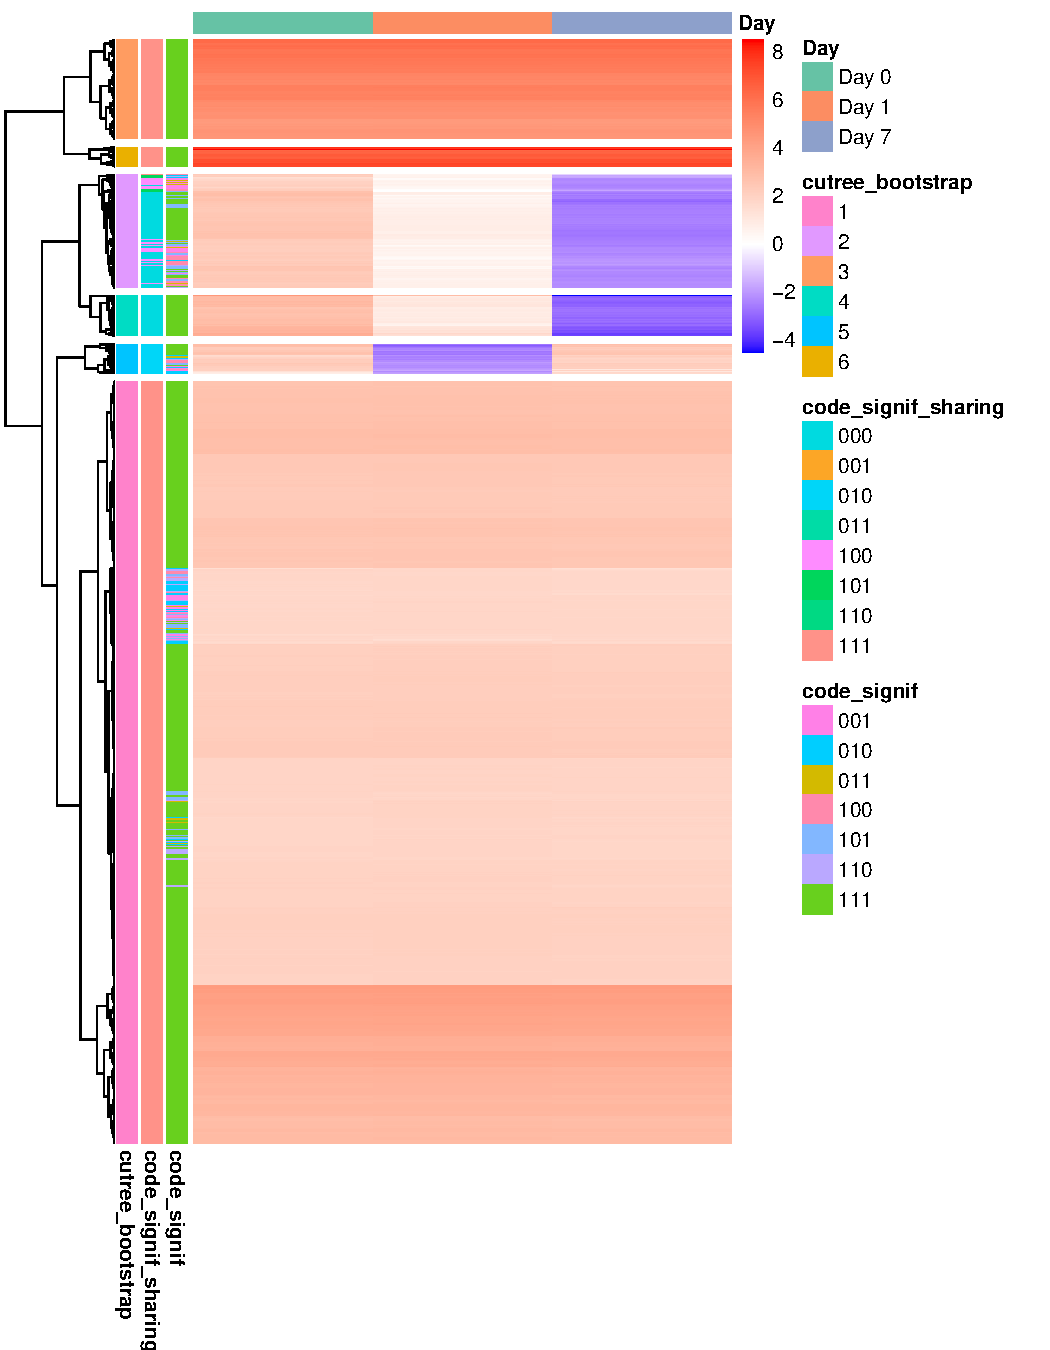
\includegraphics[width=1.0\textwidth,page=1]{mainmatter/figures/chapter_03/plot_dge_eqtl.heatmap_eqtl.pdf}
%     \caption{}
%     \label{fig:hird_eQTL_heatmap_mega}
% \end{figure}

potential problems with mega discussed b4
- platform fx
- Using a fixed effect assumes mean diff between rnaseq and array and forces the slope to the average.
- lme4qtl interactions with bonferroni

\subsection{Characterising re-eQTLs at each timepoint}

% Possible Ranking metrics:
%     PVE: prefers large maf and high betas since it squares the beta. even if the beta does not change so much. ignores sign.
%     beta:
%     p: ignores sign
%     Z score:
\missingfigure{tmod reqtls}

- DGE vs reQTL
- fisher test

- an example of d1 reQTL at adcy3

- previously found in franco
and in:
whole blood
% (A) ADCY3, (B) DNAAF1 and (C) ZNF517):
% before and after stimulation with M. leprae sonicate in whole blood cells.
% https://journals.plos.org/plosgenetics/article?id=10.1371/journal.pgen.1006952
and in: 
caliskan

and in High-throughput allele-specific expression across 250 environmental conditions
% https://www.ncbi.nlm.nih.gov/pmc/articles/PMC5131815/

- high expre at all t, so not due to cell type specific e
- not DGE either
- possible mech is cell type specific eqtl

\begin{figure}
    \centering
    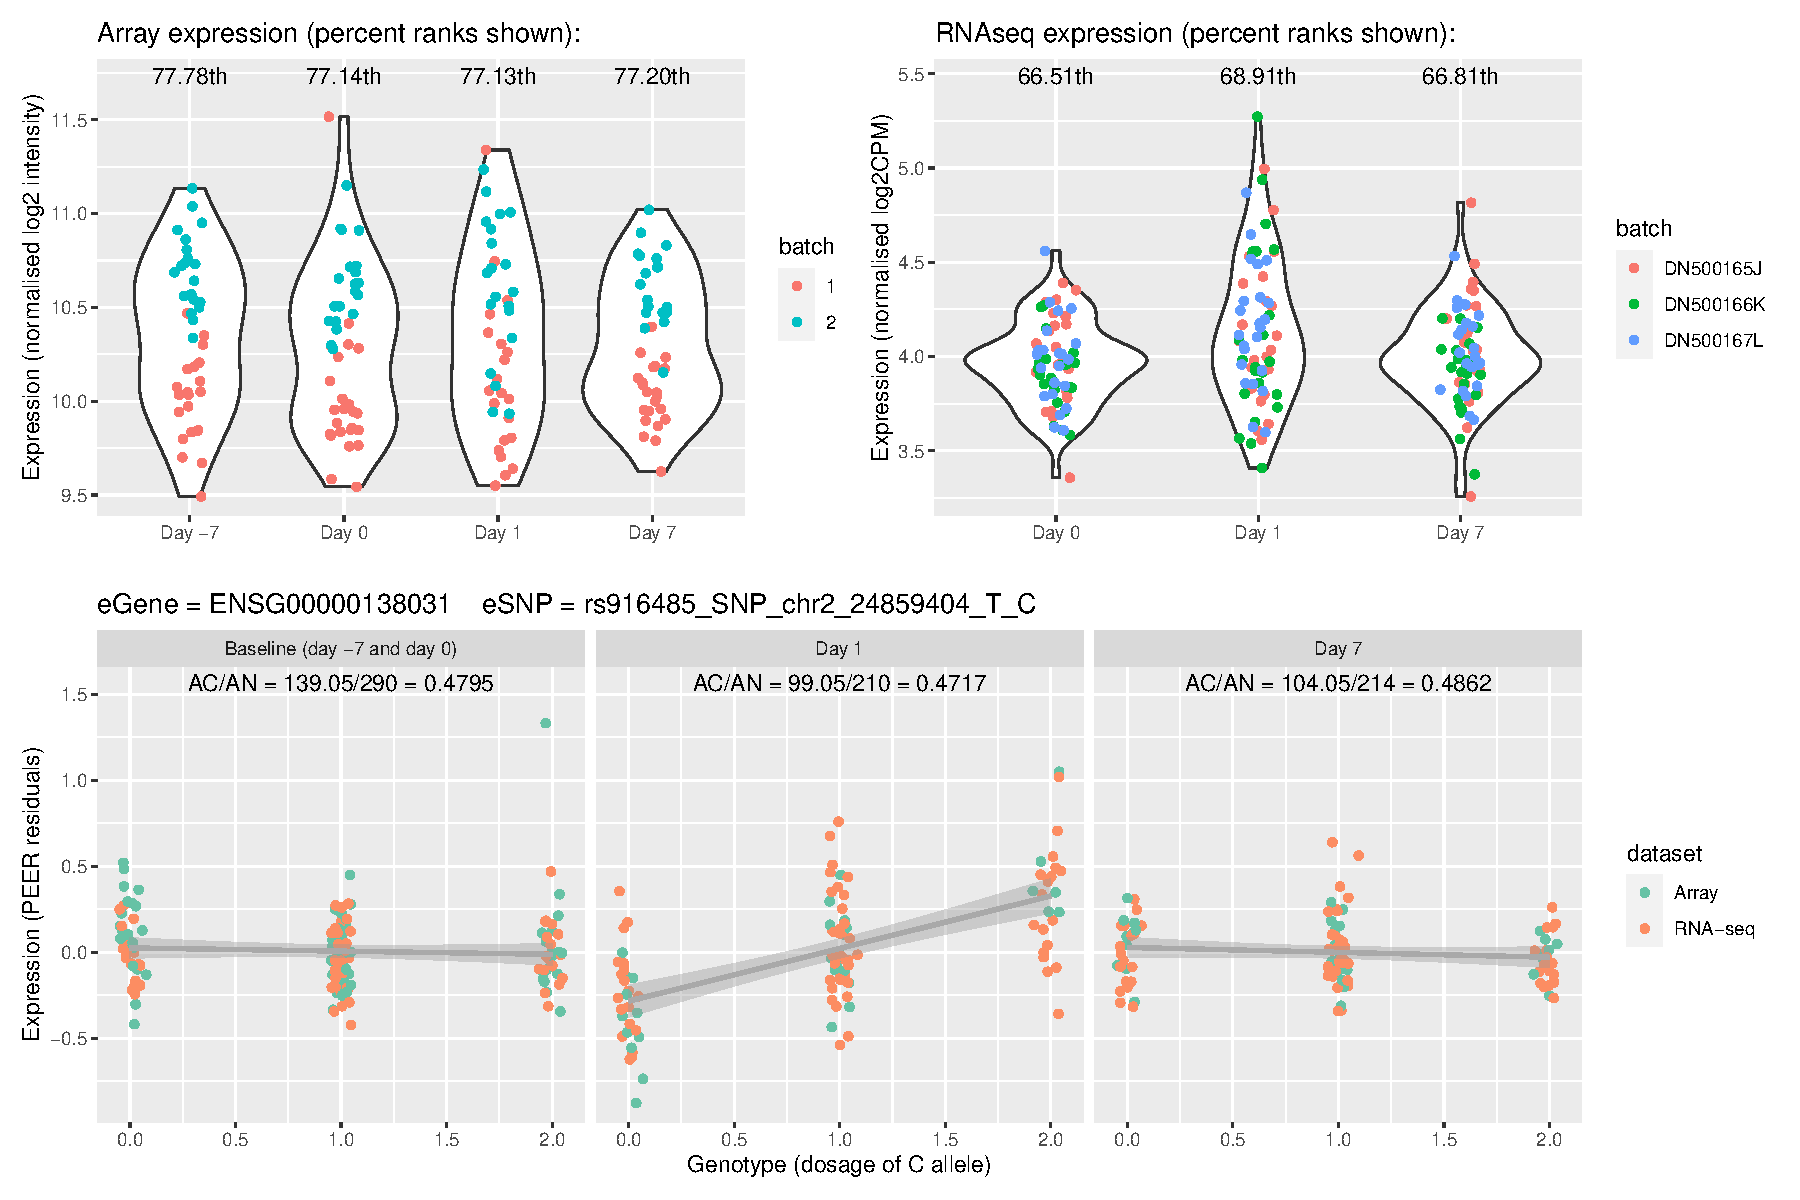
\includegraphics[width=1.0\textwidth,page=1]{mainmatter/figures/chapter_03/plot_dge_eqtl_genotypes.ENSG00000138031,rs916485_SNP_chr2_24859404_T_C.pdf}
    \caption{}
    \label{fig:hird_eQTL_ADCY3}
\end{figure}

- interaction with cell type lme4qtl

\subsection{TODO Colocalisation of re-eQTLs with known context-specific immune QTLs}

% Figure with e.g. reQTL coloc
Colocalisation with known associations;
Colocalisation is used to understand the molecular basis of GWAS associations (of a variety of human disease traits) (Giambartolome, 2014);
Here the inverse: coloc is used to understand the biological relevance of observed expression variation

% What is coloc and why coloc
% See coloc_comparisons in notes for a summary
Choice of method; 
Coloc and assumptions; Hypercoloc and assumptions

\subsection{TODO Disruption of binding site motifs as a model for reQTLs}

\section{Discussion}

more reqtls at d1, expected
Given the large changes in expression, detect context-specific fx.


How much sharing vs expected?


Biggest question remains, why are reQTLs reQTLs

Confounded by changes in immune cell proportions in bulk PBMCs;
how good is our deconv? stim at day 1
Note, the use of gene signatures for deconv
    in stimulated samples
    does not distinguish upreg from prolif either
    if expression goes up, the method will detect more of the signature
    i.e. it may correct away some signal of upregulation

assume that main effect is signif 
lme4qtl was not scalable


Why dge eqtl overlap poor?
what other mechs?

It must be said, overlap is not rigorous
Formal Mediation analysis required

Unclear connection to vaccine biology e.g. what genesets/pathways/cell types are driving the observed transcriptomic and eQTL response?;
big lim: sample size: unable to leverage Ab data for mediation analysis
misses a main advantage of in vivo design


Confounding by multiple causal variants?;
No conditional eQTL analysis to disentangle conditional effects;
miss some reQTLs
Are re qtls more likely to be distal and secondary?


